\documentclass[1p]{elsarticle_modified}
%\bibliographystyle{elsarticle-num}

%\usepackage[colorlinks]{hyperref}
%\usepackage{abbrmath_seonhwa} %\Abb, \Ascr, \Acal ,\Abf, \Afrak
\usepackage{amsfonts}
\usepackage{amssymb}
\usepackage{amsmath}
\usepackage{amsthm}
\usepackage{scalefnt}
\usepackage{amsbsy}
\usepackage{kotex}
\usepackage{caption}
\usepackage{subfig}
\usepackage{color}
\usepackage{graphicx}
\usepackage{xcolor} %% white, black, red, green, blue, cyan, magenta, yellow
\usepackage{float}
\usepackage{setspace}
\usepackage{hyperref}

\usepackage{tikz}
\usetikzlibrary{arrows}

\usepackage{multirow}
\usepackage{array} % fixed length table
\usepackage{hhline}

%%%%%%%%%%%%%%%%%%%%%
\makeatletter
\renewcommand*\env@matrix[1][\arraystretch]{%
	\edef\arraystretch{#1}%
	\hskip -\arraycolsep
	\let\@ifnextchar\new@ifnextchar
	\array{*\c@MaxMatrixCols c}}
\makeatother %https://tex.stackexchange.com/questions/14071/how-can-i-increase-the-line-spacing-in-a-matrix
%%%%%%%%%%%%%%%

\usepackage[normalem]{ulem}

\newcommand{\msout}[1]{\ifmmode\text{\sout{\ensuremath{#1}}}\else\sout{#1}\fi}
%SOURCE: \msout is \stkout macro in https://tex.stackexchange.com/questions/20609/strikeout-in-math-mode

\newcommand{\cancel}[1]{
	\ifmmode
	{\color{red}\msout{#1}}
	\else
	{\color{red}\sout{#1}}
	\fi
}

\newcommand{\add}[1]{
	{\color{blue}\uwave{#1}}
}

\newcommand{\replace}[2]{
	\ifmmode
	{\color{red}\msout{#1}}{\color{blue}\uwave{#2}}
	\else
	{\color{red}\sout{#1}}{\color{blue}\uwave{#2}}
	\fi
}

\newcommand{\Sol}{\mathcal{S}} %segment
\newcommand{\D}{D} %diagram
\newcommand{\A}{\mathcal{A}} %arc


%%%%%%%%%%%%%%%%%%%%%%%%%%%%%5 test

\def\sl{\operatorname{\textup{SL}}(2,\Cbb)}
\def\psl{\operatorname{\textup{PSL}}(2,\Cbb)}
\def\quan{\mkern 1mu \triangleright \mkern 1mu}

\theoremstyle{definition}
\newtheorem{thm}{Theorem}[section]
\newtheorem{prop}[thm]{Proposition}
\newtheorem{lem}[thm]{Lemma}
\newtheorem{ques}[thm]{Question}
\newtheorem{cor}[thm]{Corollary}
\newtheorem{defn}[thm]{Definition}
\newtheorem{exam}[thm]{Example}
\newtheorem{rmk}[thm]{Remark}
\newtheorem{alg}[thm]{Algorithm}

\newcommand{\I}{\sqrt{-1}}
\begin{document}

%\begin{frontmatter}
%
%\title{Boundary parabolic representations of knots up to 8 crossings}
%
%%% Group authors per affiliation:
%\author{Yunhi Cho} 
%\address{Department of Mathematics, University of Seoul, Seoul, Korea}
%\ead{yhcho@uos.ac.kr}
%
%
%\author{Seonhwa Kim} %\fnref{s_kim}}
%\address{Center for Geometry and Physics, Institute for Basic Science, Pohang, 37673, Korea}
%\ead{ryeona17@ibs.re.kr}
%
%\author{Hyuk Kim}
%\address{Department of Mathematical Sciences, Seoul National University, Seoul 08826, Korea}
%\ead{hyukkim@snu.ac.kr}
%
%\author{Seokbeom Yoon}
%\address{Department of Mathematical Sciences, Seoul National University, Seoul, 08826,  Korea}
%\ead{sbyoon15@snu.ac.kr}
%
%\begin{abstract}
%We find all boundary parabolic representation of knots up to 8 crossings.
%
%\end{abstract}
%\begin{keyword}
%    \MSC[2010] 57M25 
%\end{keyword}
%
%\end{frontmatter}

%\linenumbers
%\tableofcontents
%
\newcommand\colored[1]{\textcolor{white}{\rule[-0.35ex]{0.8em}{1.4ex}}\kern-0.8em\color{red} #1}%
%\newcommand\colored[1]{\textcolor{white}{ #1}\kern-2.17ex	\textcolor{white}{ #1}\kern-1.81ex	\textcolor{white}{ #1}\kern-2.15ex\color{red}#1	}

{\Large $\underline{10_{159}~(K10n_{34})}$}

\setlength{\tabcolsep}{10pt}
\renewcommand{\arraystretch}{1.6}
\vspace{1cm}\begin{tabular}{m{100pt}>{\centering\arraybackslash}m{274pt}}
\multirow{5}{120pt}{
	\centering
	\includegraphics[width=112pt]{../../../GIT/diagram.site/Diagrams/png/243_10_159.png}\\
\ \ \ A knot diagram\footnotemark}&
\allowdisplaybreaks
\textbf{Linearized knot diagam} \\
\cline{2-2}
 &
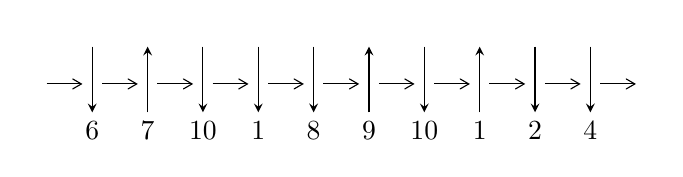
\begin{tikzpicture}[x=20pt, y=17pt]
	% nodes
	\node (C0) at (0, 0) {};
	\node (C1) at (1, 0) {};
	\node (C1U) at (1, +1) {};
	\node (C1D) at (1, -1) {6};

	\node (C2) at (2, 0) {};
	\node (C2U) at (2, +1) {};
	\node (C2D) at (2, -1) {7};

	\node (C3) at (3, 0) {};
	\node (C3U) at (3, +1) {};
	\node (C3D) at (3, -1) {10};

	\node (C4) at (4, 0) {};
	\node (C4U) at (4, +1) {};
	\node (C4D) at (4, -1) {1};

	\node (C5) at (5, 0) {};
	\node (C5U) at (5, +1) {};
	\node (C5D) at (5, -1) {8};

	\node (C6) at (6, 0) {};
	\node (C6U) at (6, +1) {};
	\node (C6D) at (6, -1) {9};

	\node (C7) at (7, 0) {};
	\node (C7U) at (7, +1) {};
	\node (C7D) at (7, -1) {10};

	\node (C8) at (8, 0) {};
	\node (C8U) at (8, +1) {};
	\node (C8D) at (8, -1) {1};

	\node (C9) at (9, 0) {};
	\node (C9U) at (9, +1) {};
	\node (C9D) at (9, -1) {2};

	\node (C10) at (10, 0) {};
	\node (C10U) at (10, +1) {};
	\node (C10D) at (10, -1) {4};
	\node (C11) at (11, 0) {};

	% arrows
	\draw[->,>={angle 60}]
	(C0) edge (C1) (C1) edge (C2) (C2) edge (C3) (C3) edge (C4) (C4) edge (C5) (C5) edge (C6) (C6) edge (C7) (C7) edge (C8) (C8) edge (C9) (C9) edge (C10) (C10) edge (C11) ;	\draw[->,>=stealth]
	(C1U) edge (C1D) (C2D) edge (C2U) (C3U) edge (C3D) (C4U) edge (C4D) (C5U) edge (C5D) (C6D) edge (C6U) (C7U) edge (C7D) (C8D) edge (C8U) (C9U) edge (C9D) (C10U) edge (C10D) ;
	\end{tikzpicture} \\
\hhline{~~} \\& 
\textbf{Solving Sequence} \\ \cline{2-2} 
 &
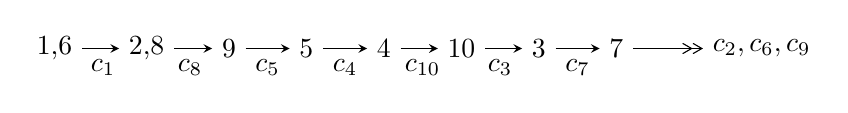
\begin{tikzpicture}[x=28pt, y=7pt]
	% node
	\node (A0) at (-1/8, 0) {1,6};
	\node (A1) at (17/16, 0) {2,8};
	\node (A2) at (17/8, 0) {9};
	\node (A3) at (25/8, 0) {5};
	\node (A4) at (33/8, 0) {4};
	\node (A5) at (41/8, 0) {10};
	\node (A6) at (49/8, 0) {3};
	\node (A7) at (57/8, 0) {7};
	\node (C1) at (1/2, -1) {$c_{1}$};
	\node (C2) at (13/8, -1) {$c_{8}$};
	\node (C3) at (21/8, -1) {$c_{5}$};
	\node (C4) at (29/8, -1) {$c_{4}$};
	\node (C5) at (37/8, -1) {$c_{10}$};
	\node (C6) at (45/8, -1) {$c_{3}$};
	\node (C7) at (53/8, -1) {$c_{7}$};
	\node (A8) at (9, 0) {$c_{2},c_{6},c_{9}$};

	% edge
	\draw[->,>=stealth]	
	(A0) edge (A1) (A1) edge (A2) (A2) edge (A3) (A3) edge (A4) (A4) edge (A5) (A5) edge (A6) (A6) edge (A7) ;
	\draw[->>,>={angle 60}]	
	(A7) edge (A8);
\end{tikzpicture} \\ 

\end{tabular} \\

\footnotetext{
The image of knot diagram is generated by the software ``\textbf{Draw programme}" developed by Andrew Bartholomew(\url{http://www.layer8.co.uk/maths/draw/index.htm\#Running-draw}), where we modified some parts for our purpose(\url{https://github.com/CATsTAILs/LinksPainter}).
}\phantom \\ \newline 
\centering \textbf{Ideals for irreducible components\footnotemark of $X_{\text{par}}$} 
 
\begin{align*}
I^u_{1}&=\langle 
-31 u^8+18 u^7+76 u^6-39 u^5-208 u^4+102 u^3+226 u^2+25 b-20 u-72,\\
\phantom{I^u_{1}}&\phantom{= \langle  }-108 u^8+49 u^7+243 u^6-77 u^5-694 u^4+261 u^3+693 u^2+25 a+65 u-196,\\
\phantom{I^u_{1}}&\phantom{= \langle  }u^9- u^8-2 u^7+2 u^6+6 u^5-6 u^4-5 u^3+3 u^2+2 u-1\rangle \\
I^u_{2}&=\langle 
1002 u^{13}-332 u^{12}+\cdots+1889 b+2916,\;-2310 u^{13}+279 u^{12}+\cdots+1889 a-9392,\\
\phantom{I^u_{2}}&\phantom{= \langle  }u^{14}+u^{11}+3 u^{10}+2 u^9-7 u^8+7 u^7- u^6+11 u^5-14 u^4+9 u^3-5 u^2+5 u-1\rangle \\
I^u_{3}&=\langle 
u^2+b-1,\;u^2+a+u,\;u^3- u+1\rangle \\
I^u_{4}&=\langle 
b- u+1,\;a+u-1,\;u^2- u-1\rangle \\
I^u_{5}&=\langle 
b+1,\;a-1,\;u+1\rangle \\
\\
\end{align*}
\raggedright * 5 irreducible components of $\dim_{\mathbb{C}}=0$, with total 29 representations.\\
\footnotetext{All coefficients of polynomials are rational numbers. But the coefficients are sometimes approximated in decimal forms when there is not enough margin.}
\newpage
\renewcommand{\arraystretch}{1}
\centering \section*{I. $I^u_{1}= \langle -31 u^8+18 u^7+\cdots+25 b-72,\;-108 u^8+49 u^7+\cdots+25 a-196,\;u^9- u^8+\cdots+2 u-1 \rangle$}
\flushleft \textbf{(i) Arc colorings}\\
\begin{tabular}{m{7pt} m{180pt} m{7pt} m{180pt} }
\flushright $a_{1}=$&$\begin{pmatrix}1\\0\end{pmatrix}$ \\
\flushright $a_{6}=$&$\begin{pmatrix}0\\u\end{pmatrix}$ \\
\flushright $a_{2}=$&$\begin{pmatrix}1\\u^2\end{pmatrix}$ \\
\flushright $a_{8}=$&$\begin{pmatrix}4.32000 u^{8}-1.96000 u^{7}+\cdots-2.60000 u+7.84000\\\frac{31}{25} u^8-\frac{18}{25} u^7+\cdots+\frac{4}{5} u+\frac{72}{25}\end{pmatrix}$ \\
\flushright $a_{9}=$&$\begin{pmatrix}5.56000 u^{8}-2.68000 u^{7}+\cdots-1.80000 u+10.7200\\\frac{31}{25} u^8-\frac{18}{25} u^7+\cdots+\frac{4}{5} u+\frac{72}{25}\end{pmatrix}$ \\
\flushright $a_{5}=$&$\begin{pmatrix}-1.76000 u^{8}+1.28000 u^{7}+\cdots-2.20000 u-5.12000\\\frac{48}{25} u^8-\frac{19}{25} u^7+\cdots-\frac{3}{5} u+\frac{76}{25}\end{pmatrix}$ \\
\flushright $a_{4}=$&$\begin{pmatrix}\frac{4}{25} u^8+\frac{13}{25} u^7+\cdots-\frac{14}{5} u-\frac{52}{25}\\\frac{48}{25} u^8-\frac{19}{25} u^7+\cdots-\frac{3}{5} u+\frac{76}{25}\end{pmatrix}$ \\
\flushright $a_{10}=$&$\begin{pmatrix}5.56000 u^{8}-2.68000 u^{7}+\cdots-2.80000 u+10.7200\\\frac{31}{25} u^8-\frac{18}{25} u^7+\cdots+\frac{4}{5} u+\frac{72}{25}\end{pmatrix}$ \\
\flushright $a_{3}=$&$\begin{pmatrix}-2.76000 u^{8}+2.28000 u^{7}+\cdots-4.20000 u-9.12000\\\frac{12}{5} u^8-\frac{6}{5} u^7+\cdots-2 u+\frac{19}{5}\end{pmatrix}$ \\
\flushright $a_{7}=$&$\begin{pmatrix}\frac{16}{5} u^8-\frac{3}{5} u^7+\cdots-6 u+\frac{17}{5}\\3.04000 u^{8}-1.12000 u^{7}+\cdots-1.20000 u+5.48000\end{pmatrix}$\\&\end{tabular}
\flushleft \textbf{(ii) Obstruction class $= -1$}\\~\\
\flushleft \textbf{(iii) Cusp Shapes $= -\frac{96}{25} u^8+\frac{13}{25} u^7+\frac{216}{25} u^6-\frac{24}{25} u^5-\frac{653}{25} u^4+\frac{82}{25} u^3+\frac{691}{25} u^2+\frac{26}{5} u-\frac{377}{25}$}\\~\\
\newpage\renewcommand{\arraystretch}{1}
\flushleft \textbf{(iv) u-Polynomials at the component}\newline \\
\begin{tabular}{m{50pt}|m{274pt}}
Crossings & \hspace{64pt}u-Polynomials at each crossing \\
\hline $$\begin{aligned}c_{1},c_{9}\end{aligned}$$&$\begin{aligned}
&u^9- u^8-2 u^7+2 u^6+6 u^5-6 u^4-5 u^3+3 u^2+2 u-1
\end{aligned}$\\
\hline $$\begin{aligned}c_{2},c_{8}\end{aligned}$$&$\begin{aligned}
&u^9-4 u^7+7 u^5-2 u^4-4 u^3- u^2+3 u+1
\end{aligned}$\\
\hline $$\begin{aligned}c_{3},c_{4},c_{10}\end{aligned}$$&$\begin{aligned}
&u^9+5 u^8+12 u^7+12 u^6-6 u^5-38 u^4-57 u^3-49 u^2-24 u-5
\end{aligned}$\\
\hline $$\begin{aligned}c_{5},c_{7}\end{aligned}$$&$\begin{aligned}
&u^9+6 u^7+4 u^6+15 u^5+18 u^4+18 u^3+19 u^2+7 u+1
\end{aligned}$\\
\hline $$\begin{aligned}c_{6}\end{aligned}$$&$\begin{aligned}
&u^9+7 u^8+22 u^7+44 u^6+72 u^5+102 u^4+103 u^3+59 u^2+18 u+5
\end{aligned}$\\
\hline
\end{tabular}\\~\\
\newpage\renewcommand{\arraystretch}{1}
\flushleft \textbf{(v) Riley Polynomials at the component}\newline \\
\begin{tabular}{m{50pt}|m{274pt}}
Crossings & \hspace{64pt}Riley Polynomials at each crossing \\
\hline $$\begin{aligned}c_{1},c_{9}\end{aligned}$$&$\begin{aligned}
&y^9-5 y^8+20 y^7-50 y^6+90 y^5-118 y^4+89 y^3-41 y^2+10 y-1
\end{aligned}$\\
\hline $$\begin{aligned}c_{2},c_{8}\end{aligned}$$&$\begin{aligned}
&y^9-8 y^8+30 y^7-64 y^6+87 y^5-84 y^4+54 y^3-21 y^2+11 y-1
\end{aligned}$\\
\hline $$\begin{aligned}c_{3},c_{4},c_{10}\end{aligned}$$&$\begin{aligned}
&y^9- y^8+12 y^7-22 y^6+22 y^5-110 y^4-67 y^3-45 y^2+86 y-25
\end{aligned}$\\
\hline $$\begin{aligned}c_{5},c_{7}\end{aligned}$$&$\begin{aligned}
&y^9+12 y^8+\cdots+11 y-1
\end{aligned}$\\
\hline $$\begin{aligned}c_{6}\end{aligned}$$&$\begin{aligned}
&y^9-5 y^8+12 y^7+10 y^6-50 y^5-42 y^4+725 y^3-793 y^2-266 y-25
\end{aligned}$\\
\hline
\end{tabular}\\~\\
\newpage\flushleft \textbf{(vi) Complex Volumes and Cusp Shapes}
$$\begin{array}{c|c|c}  
\text{Solutions to }I^u_{1}& \I (\text{vol} + \sqrt{-1}CS) & \text{Cusp shape}\\
 \hline 
\begin{aligned}
u &= -0.675360 + 0.321360 I \\
a &= \phantom{-}0.375927 - 0.035170 I \\
b &= -0.490473 + 0.554222 I\end{aligned}
 & -1.230240 + 0.388380 I & -8.56083 - 2.01333 I \\ \hline\begin{aligned}
u &= -0.675360 - 0.321360 I \\
a &= \phantom{-}0.375927 + 0.035170 I \\
b &= -0.490473 - 0.554222 I\end{aligned}
 & -1.230240 - 0.388380 I & -8.56083 + 2.01333 I \\ \hline\begin{aligned}
u &= \phantom{-}1.27629\phantom{ +0.000000I} \\
a &= -0.656695\phantom{ +0.000000I} \\
b &= -0.328475\phantom{ +0.000000I}\end{aligned}
 & -6.80161\phantom{ +0.000000I} & -15.9820\phantom{ +0.000000I} \\ \hline\begin{aligned}
u &= -1.16884 + 0.87463 I \\
a &= -0.616776 + 0.922983 I \\
b &= \phantom{-}1.299660 + 0.083541 I\end{aligned}
 & \phantom{-}5.93576 + 3.11393 I & -2.06870 - 2.32890 I \\ \hline\begin{aligned}
u &= -1.16884 - 0.87463 I \\
a &= -0.616776 - 0.922983 I \\
b &= \phantom{-}1.299660 - 0.083541 I\end{aligned}
 & \phantom{-}5.93576 - 3.11393 I & -2.06870 + 2.32890 I \\ \hline\begin{aligned}
u &= \phantom{-}0.523277 + 0.089360 I \\
a &= -0.56707 - 2.28589 I \\
b &= \phantom{-}0.883398 - 0.665684 I\end{aligned}
 & \phantom{-}0.97258 - 2.76102 I & -6.12756 + 2.10529 I \\ \hline\begin{aligned}
u &= \phantom{-}0.523277 - 0.089360 I \\
a &= -0.56707 + 2.28589 I \\
b &= \phantom{-}0.883398 + 0.665684 I\end{aligned}
 & \phantom{-}0.97258 + 2.76102 I & -6.12756 - 2.10529 I \\ \hline\begin{aligned}
u &= \phantom{-}1.18278 + 0.96607 I \\
a &= \phantom{-}1.136270 + 0.521152 I \\
b &= -1.52834 + 0.58529 I\end{aligned}
 & \phantom{-}5.94738 - 11.74060 I & -3.25195 + 6.67016 I \\ \hline\begin{aligned}
u &= \phantom{-}1.18278 - 0.96607 I \\
a &= \phantom{-}1.136270 - 0.521152 I \\
b &= -1.52834 - 0.58529 I\end{aligned}
 & \phantom{-}5.94738 + 11.74060 I & -3.25195 - 6.67016 I\\
 \hline 
 \end{array}$$\newpage\newpage\renewcommand{\arraystretch}{1}
\centering \section*{II. $I^u_{2}= \langle 1002 u^{13}-332 u^{12}+\cdots+1889 b+2916,\;-2310 u^{13}+279 u^{12}+\cdots+1889 a-9392,\;u^{14}+u^{11}+\cdots+5 u-1 \rangle$}
\flushleft \textbf{(i) Arc colorings}\\
\begin{tabular}{m{7pt} m{180pt} m{7pt} m{180pt} }
\flushright $a_{1}=$&$\begin{pmatrix}1\\0\end{pmatrix}$ \\
\flushright $a_{6}=$&$\begin{pmatrix}0\\u\end{pmatrix}$ \\
\flushright $a_{2}=$&$\begin{pmatrix}1\\u^2\end{pmatrix}$ \\
\flushright $a_{8}=$&$\begin{pmatrix}1.22287 u^{13}-0.147697 u^{12}+\cdots-5.55214 u+4.97194\\-0.530439 u^{13}+0.175754 u^{12}+\cdots+1.11223 u-1.54367\end{pmatrix}$ \\
\flushright $a_{9}=$&$\begin{pmatrix}0.692430 u^{13}+0.0280572 u^{12}+\cdots-4.43992 u+3.42827\\-0.530439 u^{13}+0.175754 u^{12}+\cdots+1.11223 u-1.54367\end{pmatrix}$ \\
\flushright $a_{5}=$&$\begin{pmatrix}0.967708 u^{13}-0.0831128 u^{12}+\cdots-6.71572 u+5.12758\\-0.582319 u^{13}-0.0725251 u^{12}+\cdots+2.92959 u-1.74854\end{pmatrix}$ \\
\flushright $a_{4}=$&$\begin{pmatrix}0.385389 u^{13}-0.155638 u^{12}+\cdots-3.78613 u+3.37904\\-0.582319 u^{13}-0.0725251 u^{12}+\cdots+2.92959 u-1.74854\end{pmatrix}$ \\
\flushright $a_{10}=$&$\begin{pmatrix}u^{13}+u^{10}+3 u^9+2 u^8-7 u^7+7 u^6- u^5+11 u^4-14 u^3+9 u^2-5 u+5\\-0.307570 u^{13}+0.0280572 u^{12}+\cdots+1.56008 u-1.57173\end{pmatrix}$ \\
\flushright $a_{3}=$&$\begin{pmatrix}-1.36316 u^{13}-0.737957 u^{12}+\cdots+1.72155 u-2.43409\\-0.238221 u^{13}+0.288512 u^{12}+\cdots+2.83483 u-0.124404\end{pmatrix}$ \\
\flushright $a_{7}=$&$\begin{pmatrix}0.592377 u^{13}+0.0492324 u^{12}+\cdots-5.14929 u+2.67602\\0.206988 u^{13}+0.204870 u^{12}+\cdots+0.636845 u-0.703017\end{pmatrix}$\\&\end{tabular}
\flushleft \textbf{(ii) Obstruction class $= -1$}\\~\\
\flushleft \textbf{(iii) Cusp Shapes $= \frac{1965}{1889} u^{13}+\frac{5491}{1889} u^{12}+\cdots-\frac{3549}{1889} u+\frac{3230}{1889}$}\\~\\
\newpage\renewcommand{\arraystretch}{1}
\flushleft \textbf{(iv) u-Polynomials at the component}\newline \\
\begin{tabular}{m{50pt}|m{274pt}}
Crossings & \hspace{64pt}u-Polynomials at each crossing \\
\hline $$\begin{aligned}c_{1},c_{9}\end{aligned}$$&$\begin{aligned}
&u^{14}+u^{11}+\cdots+5 u-1
\end{aligned}$\\
\hline $$\begin{aligned}c_{2},c_{8}\end{aligned}$$&$\begin{aligned}
&u^{14}-6 u^{12}+\cdots-9 u+1
\end{aligned}$\\
\hline $$\begin{aligned}c_{3},c_{4},c_{10}\end{aligned}$$&$\begin{aligned}
&(u^7-2 u^6+2 u^5+u^4-2 u^3+3 u^2-2 u+1)^2
\end{aligned}$\\
\hline $$\begin{aligned}c_{5},c_{7}\end{aligned}$$&$\begin{aligned}
&u^{14}-3 u^{13}+\cdots-6 u-1
\end{aligned}$\\
\hline $$\begin{aligned}c_{6}\end{aligned}$$&$\begin{aligned}
&(u^7-3 u^6+3 u^5+2 u^4-6 u^3+3 u^2+3 u-2)^2
\end{aligned}$\\
\hline
\end{tabular}\\~\\
\newpage\renewcommand{\arraystretch}{1}
\flushleft \textbf{(v) Riley Polynomials at the component}\newline \\
\begin{tabular}{m{50pt}|m{274pt}}
Crossings & \hspace{64pt}Riley Polynomials at each crossing \\
\hline $$\begin{aligned}c_{1},c_{9}\end{aligned}$$&$\begin{aligned}
&y^{14}+6 y^{12}+\cdots-15 y+1
\end{aligned}$\\
\hline $$\begin{aligned}c_{2},c_{8}\end{aligned}$$&$\begin{aligned}
&y^{14}-12 y^{13}+\cdots-63 y+1
\end{aligned}$\\
\hline $$\begin{aligned}c_{3},c_{4},c_{10}\end{aligned}$$&$\begin{aligned}
&(y^7+4 y^5- y^4-6 y^3-3 y^2-2 y-1)^2
\end{aligned}$\\
\hline $$\begin{aligned}c_{5},c_{7}\end{aligned}$$&$\begin{aligned}
&y^{14}+13 y^{13}+\cdots+42 y+1
\end{aligned}$\\
\hline $$\begin{aligned}c_{6}\end{aligned}$$&$\begin{aligned}
&(y^7-3 y^6+9 y^5-16 y^4+30 y^3-37 y^2+21 y-4)^2
\end{aligned}$\\
\hline
\end{tabular}\\~\\
\newpage\flushleft \textbf{(vi) Complex Volumes and Cusp Shapes}
$$\begin{array}{c|c|c}  
\text{Solutions to }I^u_{2}& \I (\text{vol} + \sqrt{-1}CS) & \text{Cusp shape}\\
 \hline 
\begin{aligned}
u &= \phantom{-}0.877499 + 0.643882 I \\
a &= -0.815701 - 0.730313 I \\
b &= \phantom{-}1.36033 - 0.47577 I\end{aligned}
 & \phantom{-}2.12977 - 2.53884 I & \phantom{-}0.86344 + 1.81085 I \\ \hline\begin{aligned}
u &= \phantom{-}0.877499 - 0.643882 I \\
a &= -0.815701 + 0.730313 I \\
b &= \phantom{-}1.36033 + 0.47577 I\end{aligned}
 & \phantom{-}2.12977 + 2.53884 I & \phantom{-}0.86344 - 1.81085 I \\ \hline\begin{aligned}
u &= \phantom{-}0.763487 + 0.442848 I \\
a &= -0.149425 - 0.086700 I \\
b &= \phantom{-}0.33250 - 1.47887 I\end{aligned}
 & \phantom{-}0.33600 - 4.72329 I & -7.01907 + 9.17288 I \\ \hline\begin{aligned}
u &= \phantom{-}0.763487 - 0.442848 I \\
a &= -0.149425 + 0.086700 I \\
b &= \phantom{-}0.33250 + 1.47887 I\end{aligned}
 & \phantom{-}0.33600 + 4.72329 I & -7.01907 - 9.17288 I \\ \hline\begin{aligned}
u &= -0.796980 + 0.997104 I \\
a &= \phantom{-}1.285810 - 0.554607 I \\
b &= -1.011450 - 0.500189 I\end{aligned}
 & \phantom{-}0.33600 + 4.72329 I & -7.01907 - 9.17288 I \\ \hline\begin{aligned}
u &= -0.796980 - 0.997104 I \\
a &= \phantom{-}1.285810 + 0.554607 I \\
b &= -1.011450 + 0.500189 I\end{aligned}
 & \phantom{-}0.33600 - 4.72329 I & -7.01907 + 9.17288 I \\ \hline\begin{aligned}
u &= -0.775231 + 1.031020 I \\
a &= -1.276240 + 0.214140 I \\
b &= \phantom{-}1.62238 + 0.39283 I\end{aligned}
 & \phantom{-}7.17429 + 3.91715 I & -1.20398 - 3.00324 I \\ \hline\begin{aligned}
u &= -0.775231 - 1.031020 I \\
a &= -1.276240 - 0.214140 I \\
b &= \phantom{-}1.62238 - 0.39283 I\end{aligned}
 & \phantom{-}7.17429 - 3.91715 I & -1.20398 + 3.00324 I \\ \hline\begin{aligned}
u &= -0.196138 + 0.662538 I \\
a &= \phantom{-}0.30408 - 2.08007 I \\
b &= \phantom{-}0.162591 + 0.048461 I\end{aligned}
 & \phantom{-}2.12977 + 2.53884 I & \phantom{-}0.86344 - 1.81085 I \\ \hline\begin{aligned}
u &= -0.196138 - 0.662538 I \\
a &= \phantom{-}0.30408 + 2.08007 I \\
b &= \phantom{-}0.162591 - 0.048461 I\end{aligned}
 & \phantom{-}2.12977 - 2.53884 I & \phantom{-}0.86344 + 1.81085 I\\
 \hline 
 \end{array}$$\newpage$$\begin{array}{c|c|c}  
\text{Solutions to }I^u_{2}& \I (\text{vol} + \sqrt{-1}CS) & \text{Cusp shape}\\
 \hline 
\begin{aligned}
u &= \phantom{-}0.81203 + 1.22658 I \\
a &= \phantom{-}0.961913 + 0.622177 I \\
b &= -1.361880 - 0.158001 I\end{aligned}
 & \phantom{-}7.17429 + 3.91715 I & -1.20398 - 3.00324 I \\ \hline\begin{aligned}
u &= \phantom{-}0.81203 - 1.22658 I \\
a &= \phantom{-}0.961913 - 0.622177 I \\
b &= -1.361880 + 0.158001 I\end{aligned}
 & \phantom{-}7.17429 - 3.91715 I & -1.20398 + 3.00324 I \\ \hline\begin{aligned}
u &= -1.60968\phantom{ +0.000000I} \\
a &= \phantom{-}0.365698\phantom{ +0.000000I} \\
b &= -0.746600\phantom{ +0.000000I}\end{aligned}
 & -2.83077\phantom{ +0.000000I} & \phantom{-}1.71920\phantom{ +0.000000I} \\ \hline\begin{aligned}
u &= \phantom{-}0.240340\phantom{ +0.000000I} \\
a &= \phantom{-}4.01341\phantom{ +0.000000I} \\
b &= -1.46232\phantom{ +0.000000I}\end{aligned}
 & -2.83077\phantom{ +0.000000I} & \phantom{-}1.71920\phantom{ +0.000000I}\\
 \hline 
 \end{array}$$\newpage\newpage\renewcommand{\arraystretch}{1}
\centering \section*{III. $I^u_{3}= \langle u^2+b-1,\;u^2+a+u,\;u^3- u+1 \rangle$}
\flushleft \textbf{(i) Arc colorings}\\
\begin{tabular}{m{7pt} m{180pt} m{7pt} m{180pt} }
\flushright $a_{1}=$&$\begin{pmatrix}1\\0\end{pmatrix}$ \\
\flushright $a_{6}=$&$\begin{pmatrix}0\\u\end{pmatrix}$ \\
\flushright $a_{2}=$&$\begin{pmatrix}1\\u^2\end{pmatrix}$ \\
\flushright $a_{8}=$&$\begin{pmatrix}- u^2- u\\- u^2+1\end{pmatrix}$ \\
\flushright $a_{9}=$&$\begin{pmatrix}-2 u^2- u+1\\- u^2+1\end{pmatrix}$ \\
\flushright $a_{5}=$&$\begin{pmatrix}u^2-2\\- u^2\end{pmatrix}$ \\
\flushright $a_{4}=$&$\begin{pmatrix}-2\\- u^2\end{pmatrix}$ \\
\flushright $a_{10}=$&$\begin{pmatrix}-2 u^2+1\\- u^2+u\end{pmatrix}$ \\
\flushright $a_{3}=$&$\begin{pmatrix}u^2-2 u-2\\-2 u+1\end{pmatrix}$ \\
\flushright $a_{7}=$&$\begin{pmatrix}-2 u^2-2 u-1\\-2 u^2+1\end{pmatrix}$\\&\end{tabular}
\flushleft \textbf{(ii) Obstruction class $= 1$}\\~\\
\flushleft \textbf{(iii) Cusp Shapes $= 6 u^2+5 u-6$}\\~\\
\newpage\renewcommand{\arraystretch}{1}
\flushleft \textbf{(iv) u-Polynomials at the component}\newline \\
\begin{tabular}{m{50pt}|m{274pt}}
Crossings & \hspace{64pt}u-Polynomials at each crossing \\
\hline $$\begin{aligned}c_{1},c_{9}\end{aligned}$$&$\begin{aligned}
&u^3- u+1
\end{aligned}$\\
\hline $$\begin{aligned}c_{2},c_{8}\end{aligned}$$&$\begin{aligned}
&u^3+u^2-1
\end{aligned}$\\
\hline $$\begin{aligned}c_{3},c_{4}\end{aligned}$$&$\begin{aligned}
&u^3-2 u^2+u-1
\end{aligned}$\\
\hline $$\begin{aligned}c_{5},c_{7}\end{aligned}$$&$\begin{aligned}
&u^3+u^2+2 u+1
\end{aligned}$\\
\hline $$\begin{aligned}c_{6}\end{aligned}$$&$\begin{aligned}
&u^3+4 u^2+7 u+5
\end{aligned}$\\
\hline $$\begin{aligned}c_{10}\end{aligned}$$&$\begin{aligned}
&u^3+2 u^2+u+1
\end{aligned}$\\
\hline
\end{tabular}\\~\\
\newpage\renewcommand{\arraystretch}{1}
\flushleft \textbf{(v) Riley Polynomials at the component}\newline \\
\begin{tabular}{m{50pt}|m{274pt}}
Crossings & \hspace{64pt}Riley Polynomials at each crossing \\
\hline $$\begin{aligned}c_{1},c_{9}\end{aligned}$$&$\begin{aligned}
&y^3-2 y^2+y-1
\end{aligned}$\\
\hline $$\begin{aligned}c_{2},c_{8}\end{aligned}$$&$\begin{aligned}
&y^3- y^2+2 y-1
\end{aligned}$\\
\hline $$\begin{aligned}c_{3},c_{4},c_{10}\end{aligned}$$&$\begin{aligned}
&y^3-2 y^2-3 y-1
\end{aligned}$\\
\hline $$\begin{aligned}c_{5},c_{7}\end{aligned}$$&$\begin{aligned}
&y^3+3 y^2+2 y-1
\end{aligned}$\\
\hline $$\begin{aligned}c_{6}\end{aligned}$$&$\begin{aligned}
&y^3-2 y^2+9 y-25
\end{aligned}$\\
\hline
\end{tabular}\\~\\
\newpage\flushleft \textbf{(vi) Complex Volumes and Cusp Shapes}
$$\begin{array}{c|c|c}  
\text{Solutions to }I^u_{3}& \I (\text{vol} + \sqrt{-1}CS) & \text{Cusp shape}\\
 \hline 
\begin{aligned}
u &= \phantom{-}0.662359 + 0.562280 I \\
a &= -0.78492 - 1.30714 I \\
b &= \phantom{-}0.877439 - 0.744862 I\end{aligned}
 & \phantom{-}1.45094 - 3.77083 I & -1.95284 + 7.28057 I \\ \hline\begin{aligned}
u &= \phantom{-}0.662359 - 0.562280 I \\
a &= -0.78492 + 1.30714 I \\
b &= \phantom{-}0.877439 + 0.744862 I\end{aligned}
 & \phantom{-}1.45094 + 3.77083 I & -1.95284 - 7.28057 I \\ \hline\begin{aligned}
u &= -1.32472\phantom{ +0.000000I} \\
a &= -0.430160\phantom{ +0.000000I} \\
b &= -0.754878\phantom{ +0.000000I}\end{aligned}
 & -6.19175\phantom{ +0.000000I} & -2.09430\phantom{ +0.000000I}\\
 \hline 
 \end{array}$$\newpage\newpage\renewcommand{\arraystretch}{1}
\centering \section*{IV. $I^u_{4}= \langle b- u+1,\;a+u-1,\;u^2- u-1 \rangle$}
\flushleft \textbf{(i) Arc colorings}\\
\begin{tabular}{m{7pt} m{180pt} m{7pt} m{180pt} }
\flushright $a_{1}=$&$\begin{pmatrix}1\\0\end{pmatrix}$ \\
\flushright $a_{6}=$&$\begin{pmatrix}0\\u\end{pmatrix}$ \\
\flushright $a_{2}=$&$\begin{pmatrix}1\\u+1\end{pmatrix}$ \\
\flushright $a_{8}=$&$\begin{pmatrix}- u+1\\u-1\end{pmatrix}$ \\
\flushright $a_{9}=$&$\begin{pmatrix}0\\u-1\end{pmatrix}$ \\
\flushright $a_{5}=$&$\begin{pmatrix}u-1\\1\end{pmatrix}$ \\
\flushright $a_{4}=$&$\begin{pmatrix}u\\1\end{pmatrix}$ \\
\flushright $a_{10}=$&$\begin{pmatrix}- u+1\\-1\end{pmatrix}$ \\
\flushright $a_{3}=$&$\begin{pmatrix}1\\0\end{pmatrix}$ \\
\flushright $a_{7}=$&$\begin{pmatrix}0\\u\end{pmatrix}$\\&\end{tabular}
\flushleft \textbf{(ii) Obstruction class $= 1$}\\~\\
\flushleft \textbf{(iii) Cusp Shapes $= -17$}\\~\\
\newpage\renewcommand{\arraystretch}{1}
\flushleft \textbf{(iv) u-Polynomials at the component}\newline \\
\begin{tabular}{m{50pt}|m{274pt}}
Crossings & \hspace{64pt}u-Polynomials at each crossing \\
\hline $$\begin{aligned}c_{1},c_{2},c_{8}\\c_{9}\end{aligned}$$&$\begin{aligned}
&u^2- u-1
\end{aligned}$\\
\hline $$\begin{aligned}c_{3},c_{4}\end{aligned}$$&$\begin{aligned}
&(u+1)^2
\end{aligned}$\\
\hline $$\begin{aligned}c_{5},c_{7},c_{10}\end{aligned}$$&$\begin{aligned}
&(u-1)^2
\end{aligned}$\\
\hline $$\begin{aligned}c_{6}\end{aligned}$$&$\begin{aligned}
&u^2
\end{aligned}$\\
\hline
\end{tabular}\\~\\
\newpage\renewcommand{\arraystretch}{1}
\flushleft \textbf{(v) Riley Polynomials at the component}\newline \\
\begin{tabular}{m{50pt}|m{274pt}}
Crossings & \hspace{64pt}Riley Polynomials at each crossing \\
\hline $$\begin{aligned}c_{1},c_{2},c_{8}\\c_{9}\end{aligned}$$&$\begin{aligned}
&y^2-3 y+1
\end{aligned}$\\
\hline $$\begin{aligned}c_{3},c_{4},c_{5}\\c_{7},c_{10}\end{aligned}$$&$\begin{aligned}
&(y-1)^2
\end{aligned}$\\
\hline $$\begin{aligned}c_{6}\end{aligned}$$&$\begin{aligned}
&y^2
\end{aligned}$\\
\hline
\end{tabular}\\~\\
\newpage\flushleft \textbf{(vi) Complex Volumes and Cusp Shapes}
$$\begin{array}{c|c|c}  
\text{Solutions to }I^u_{4}& \I (\text{vol} + \sqrt{-1}CS) & \text{Cusp shape}\\
 \hline 
\begin{aligned}
u &= -0.618034\phantom{ +0.000000I} \\
a &= \phantom{-}1.61803\phantom{ +0.000000I} \\
b &= -1.61803\phantom{ +0.000000I}\end{aligned}
 & -3.28987\phantom{ +0.000000I} & -17.0000\phantom{ +0.000000I} \\ \hline\begin{aligned}
u &= \phantom{-}1.61803\phantom{ +0.000000I} \\
a &= -0.618034\phantom{ +0.000000I} \\
b &= \phantom{-}0.618034\phantom{ +0.000000I}\end{aligned}
 & -3.28987\phantom{ +0.000000I} & -17.0000\phantom{ +0.000000I}\\
 \hline 
 \end{array}$$\newpage\newpage\renewcommand{\arraystretch}{1}
\centering \section*{V. $I^u_{5}= \langle b+1,\;a-1,\;u+1 \rangle$}
\flushleft \textbf{(i) Arc colorings}\\
\begin{tabular}{m{7pt} m{180pt} m{7pt} m{180pt} }
\flushright $a_{1}=$&$\begin{pmatrix}1\\0\end{pmatrix}$ \\
\flushright $a_{6}=$&$\begin{pmatrix}0\\-1\end{pmatrix}$ \\
\flushright $a_{2}=$&$\begin{pmatrix}1\\1\end{pmatrix}$ \\
\flushright $a_{8}=$&$\begin{pmatrix}1\\-1\end{pmatrix}$ \\
\flushright $a_{9}=$&$\begin{pmatrix}0\\-1\end{pmatrix}$ \\
\flushright $a_{5}=$&$\begin{pmatrix}-1\\0\end{pmatrix}$ \\
\flushright $a_{4}=$&$\begin{pmatrix}-1\\0\end{pmatrix}$ \\
\flushright $a_{10}=$&$\begin{pmatrix}1\\0\end{pmatrix}$ \\
\flushright $a_{3}=$&$\begin{pmatrix}-1\\0\end{pmatrix}$ \\
\flushright $a_{7}=$&$\begin{pmatrix}0\\-1\end{pmatrix}$\\&\end{tabular}
\flushleft \textbf{(ii) Obstruction class $= -1$}\\~\\
\flushleft \textbf{(iii) Cusp Shapes $= -6$}\\~\\
\newpage\renewcommand{\arraystretch}{1}
\flushleft \textbf{(iv) u-Polynomials at the component}\newline \\
\begin{tabular}{m{50pt}|m{274pt}}
Crossings & \hspace{64pt}u-Polynomials at each crossing \\
\hline $$\begin{aligned}c_{1},c_{2},c_{5}\\c_{7},c_{8},c_{9}\end{aligned}$$&$\begin{aligned}
&u+1
\end{aligned}$\\
\hline $$\begin{aligned}c_{3},c_{4},c_{6}\\c_{10}\end{aligned}$$&$\begin{aligned}
&u
\end{aligned}$\\
\hline
\end{tabular}\\~\\
\newpage\renewcommand{\arraystretch}{1}
\flushleft \textbf{(v) Riley Polynomials at the component}\newline \\
\begin{tabular}{m{50pt}|m{274pt}}
Crossings & \hspace{64pt}Riley Polynomials at each crossing \\
\hline $$\begin{aligned}c_{1},c_{2},c_{5}\\c_{7},c_{8},c_{9}\end{aligned}$$&$\begin{aligned}
&y-1
\end{aligned}$\\
\hline $$\begin{aligned}c_{3},c_{4},c_{6}\\c_{10}\end{aligned}$$&$\begin{aligned}
&y
\end{aligned}$\\
\hline
\end{tabular}\\~\\
\newpage\flushleft \textbf{(vi) Complex Volumes and Cusp Shapes}
$$\begin{array}{c|c|c}  
\text{Solutions to }I^u_{5}& \I (\text{vol} + \sqrt{-1}CS) & \text{Cusp shape}\\
 \hline 
\begin{aligned}
u &= -1.00000\phantom{ +0.000000I} \\
a &= \phantom{-}1.00000\phantom{ +0.000000I} \\
b &= -1.00000\phantom{ +0.000000I}\end{aligned}
 & -1.64493\phantom{ +0.000000I} & -6.00000\phantom{ +0.000000I}\\
 \hline 
 \end{array}$$\newpage
\newpage\renewcommand{\arraystretch}{1}
\centering \section*{ VI. u-Polynomials}
\begin{tabular}{m{50pt}|m{274pt}}
Crossings & \hspace{64pt}u-Polynomials at each crossing \\
\hline $$\begin{aligned}c_{1},c_{9}\end{aligned}$$&$\begin{aligned}
&(u+1)(u^2- u-1)(u^3- u+1)\\
&\cdot(u^9- u^8-2 u^7+2 u^6+6 u^5-6 u^4-5 u^3+3 u^2+2 u-1)\\
&\cdot(u^{14}+u^{11}+\cdots+5 u-1)
\end{aligned}$\\
\hline $$\begin{aligned}c_{2},c_{8}\end{aligned}$$&$\begin{aligned}
&(u+1)(u^2- u-1)(u^3+u^2-1)(u^{9}-4 u^{7}+\cdots+3 u+1)\\
&\cdot(u^{14}-6 u^{12}+\cdots-9 u+1)
\end{aligned}$\\
\hline $$\begin{aligned}c_{3},c_{4}\end{aligned}$$&$\begin{aligned}
&u(u+1)^2(u^3-2 u^2+u-1)\\
&\cdot(u^7-2 u^6+2 u^5+u^4-2 u^3+3 u^2-2 u+1)^2\\
&\cdot(u^9+5 u^8+12 u^7+12 u^6-6 u^5-38 u^4-57 u^3-49 u^2-24 u-5)
\end{aligned}$\\
\hline $$\begin{aligned}c_{5},c_{7}\end{aligned}$$&$\begin{aligned}
&(u-1)^2(u+1)(u^3+u^2+2 u+1)\\
&\cdot(u^9+6 u^7+4 u^6+15 u^5+18 u^4+18 u^3+19 u^2+7 u+1)\\
&\cdot(u^{14}-3 u^{13}+\cdots-6 u-1)
\end{aligned}$\\
\hline $$\begin{aligned}c_{6}\end{aligned}$$&$\begin{aligned}
&u^3(u^3+4 u^2+7 u+5)(u^7-3 u^6+3 u^5+2 u^4-6 u^3+3 u^2+3 u-2)^2\\
&\cdot(u^9+7 u^8+22 u^7+44 u^6+72 u^5+102 u^4+103 u^3+59 u^2+18 u+5)
\end{aligned}$\\
\hline $$\begin{aligned}c_{10}\end{aligned}$$&$\begin{aligned}
&u(u-1)^2(u^3+2 u^2+u+1)\\
&\cdot(u^7-2 u^6+2 u^5+u^4-2 u^3+3 u^2-2 u+1)^2\\
&\cdot(u^9+5 u^8+12 u^7+12 u^6-6 u^5-38 u^4-57 u^3-49 u^2-24 u-5)
\end{aligned}$\\
\hline
\end{tabular}\newpage\renewcommand{\arraystretch}{1}
\centering \section*{ VII. Riley Polynomials}
\begin{tabular}{m{50pt}|m{274pt}}
Crossings & \hspace{64pt}Riley Polynomials at each crossing \\
\hline $$\begin{aligned}c_{1},c_{9}\end{aligned}$$&$\begin{aligned}
&(y-1)(y^2-3 y+1)(y^3-2 y^2+y-1)\\
&\cdot(y^9-5 y^8+20 y^7-50 y^6+90 y^5-118 y^4+89 y^3-41 y^2+10 y-1)\\
&\cdot(y^{14}+6 y^{12}+\cdots-15 y+1)
\end{aligned}$\\
\hline $$\begin{aligned}c_{2},c_{8}\end{aligned}$$&$\begin{aligned}
&(y-1)(y^2-3 y+1)(y^3- y^2+2 y-1)\\
&\cdot(y^9-8 y^8+30 y^7-64 y^6+87 y^5-84 y^4+54 y^3-21 y^2+11 y-1)\\
&\cdot(y^{14}-12 y^{13}+\cdots-63 y+1)
\end{aligned}$\\
\hline $$\begin{aligned}c_{3},c_{4},c_{10}\end{aligned}$$&$\begin{aligned}
&y(y-1)^2(y^3-2 y^2-3 y-1)(y^7+4 y^5- y^4-6 y^3-3 y^2-2 y-1)^2\\
&\cdot(y^9- y^8+12 y^7-22 y^6+22 y^5-110 y^4-67 y^3-45 y^2+86 y-25)
\end{aligned}$\\
\hline $$\begin{aligned}c_{5},c_{7}\end{aligned}$$&$\begin{aligned}
&((y-1)^3)(y^3+3 y^2+2 y-1)(y^9+12 y^8+\cdots+11 y-1)\\
&\cdot(y^{14}+13 y^{13}+\cdots+42 y+1)
\end{aligned}$\\
\hline $$\begin{aligned}c_{6}\end{aligned}$$&$\begin{aligned}
&y^3(y^3-2 y^2+9 y-25)\\
&\cdot(y^7-3 y^6+9 y^5-16 y^4+30 y^3-37 y^2+21 y-4)^2\\
&\cdot(y^9-5 y^8+12 y^7+10 y^6-50 y^5-42 y^4+725 y^3-793 y^2-266 y-25)
\end{aligned}$\\
\hline
\end{tabular}
\vskip 2pc
\end{document}